\chapter{Symmetry and SAT}\label{chap:symmetryinsat}


Despite SAT solving is an NP complete algorithm it works well on many real industrial problems. This is 
principally due to capacity to cut off search space with learning clause. Another ways to cut off 
search space is the exploitation of symmetry. Some instances exhibit symmetries and not taking them into account 
forces solvers to needlessly explore isomorphic search space.  \hakan{symmetrie leaves object invariant}




\section{Groups basics}

As symmetries is a belongs to a branch of mathematics called theory group.
This section give us an overview of group theory.


\subsection{Groups}

A \emph{group} is a structure $\langle G, * \rangle$, where $G$ is a non empty set and $*$ a binary
operation such the following axioms are satisfied:
\begin{itemize}[noitemsep,nolistsep]
	\item \emph{associativity}: $\forall a, b, c \in G, (a * b) * c = a * (b * c)$
	\item \emph{closure}: $\forall a, b \in G, a * b \in G$.
	\item \emph{identity}: $\forall a \in G, \exists e$ such that $ a * e = e * a = a$
	\item \emph{inverse}:  $\forall a \in G, \exists b \in G$, commonly denoted $a^{-1}$ such that
	$a * a^{-1} = a^{-1} * a = e$
\end{itemize}

Note that \emph{commutativity} is not required i.e $\ a * b = b * a$, for $a, b \in G$.
The group is \emph{abelian} if it satisfies the commutativity rule.
Moreover, the last definition leads to important properties which are: i) uniqueness of the identity element. 
To prove this property, assume $\langle G, * \rangle$ a group with two identity elements $e$ and $f$ 
then $ e = e * f = f$.
ii) uniqueness of the inverse element. To prove this property, suppose that an element $x_1$ has two inverses,
denoted $b$ and $c$ in group $\langle G, * \rangle$, then\\
 $\begin{array}{lcll}					
b & = & b * e & \\
& = & b * (a * c) & c \text{ is an inverse of } a, \text{so } e = a * c\\
& = & (b * a) * c &   \text{\emph{associativity} rule}\\
& = & e * c       & b \text{ is an inverse of } a, \text{so } e = a * b\\
& = & c           &   \text{\emph{identity} rule}
\end{array}$

The structure $\langle G, * \rangle$ is denoted as G when clear from context that G is a group
with a binary operation. In this thesis, we interested only with the \emph{finite} groups i.e
with a finite number of elements.

Given a group $G$, a \emph{subgroup} is a non empty subset of $G$ which is also a group with 
the same binary operation. If $H$ is a subgroup of $G$, we denote as $H \leq G$.
A group has at least two subgroups: i) the subgroup composed by identity element $\{e\}$, denoted \emph{trivial} subgroup.
All other subgroups are \emph{nontrivial}; ii) the subgroup composed by itself,
denoted \emph{improper} subgroup. All other subgroups are \emph{proper}.


\subsubsection{Generators of a group}

If every elements in a group G can be expressed as a linear combination
of a set of group of elements S = $\{g_1, g_2, ..., g_n \}$ then we say G is 
generated by the S. we denote this as G = $\langle S \rangle$ =
$\langle \{g_1, g_2, ..., g_n \} \rangle$ 



\subsection{Permutation groups}

A \emph{permutation} is a bijection from a set $X$ to itself.\\
Example: given a set $X = \{x_1, x_2, x_3, x_4, x_5, x_6\}$,
\begin{center}
$g = ${\Bigg( \begin{tabular}{cccccc}
		$x_1$ & $x_2$ & $x_3$ & $x_4$ & $x_5$ & $x_6$\\
		$x_2$ & $x_3$ & $x_1$ & $x_4$ & $x_6$ & $x_5$
	\end{tabular} \Bigg)}\\
\end{center}

$g$ is a permutation that maps $x_1$ to $x_2$, $x_2$ to $x_3$, $x_3$ to $x_1$, $x_4$ to $x_4$, $x_5$ to $x_6$ and $x_6$ to $x_5$.

Permutations are generally written in \emph{cycle notation}, the self mapped elements are omitted.
So the permutation in cycle notation will be : 
\begin{center}
	$g$ = ($x_1 \enskip x_2 \enskip x_3$) ($x_5 \enskip x_6$)
\end{center}

We say \emph{support} of the permutation $g$ noted $\support_{g}$ the elements that not mapped to themselves:
\begin{center}
	$\support_{g} = \{ x \in X \mid g.x \neq x\}$
\end{center}
A variable $x$ is \emph{stable} by a permutation $g$ 
if $x \notin \support_g$. A clause $\omega$ is \emph{stabilized} by a permutation $g$ if 
$\omega \cap \support_g = \emptyset$.


A set of permutations of a given set $X$ form a group $G$,
with the composition operation ($\circ$) and is called \emph{permutation group}.
The \emph{symmetric group} is the set of all possible permutations of a set $X$ and noted \Group($X$).
%The set of \textbf{all} permutations of a set $X$ is the \emph{symmetric group} of $X$ and noted \Group($X$).
So, a \emph{permutation group} is a subgroup of \Group($X$). 
%A set of permutations $P$ is a set of \emph{generators} of a group $G$ if each permutation of $G$
%can be expressed as a composition of permutations in $P$. 


A permutation group $G$ induces an \emph{equivalence relation} on the set of element $X$ being
permuted. Two elements $x_1, x_2 \in X$ are equivalent if there exists a permutation $g \in G$ such that
$g.x_1 = x_2$. Equivalence relations partition $X$ into \emph{equivalence classes} referred to
as the \emph{orbits} of $X$ under $G$. The orbit of an element $x$ under group $G$ (or simply orbit of $x$ when clear
from the context) is the set $[x]_G = \{g.x \mid g \in G\}$


\section{Symmetries in SAT}

The previous mathematical definitions of group theory is applied to the CNF formula.
The symmetric group of permutations of $\Vars$ (i.e. bijections from $\Vars$ to $\Vars$) is noted
$\Group(\Vars)$. The group $\Group(\Vars)$ naturally acts on the set of literals: for $g
\in \Group(\Vars)$ and a literal $\ell \in \Lits $, $g.\ell = g(\ell)$ if $\ell$ is a
positive literal, $g.\ell = \neg g(\neg \ell)$ if $\ell$ is a negative literal.
The group $\Group(\Vars)$ also acts on  assignments possibly partial of $\Vars$ as follows: 
\begin{center}
	$\forall g \in \Group(\Vars)$, $\alpha \in \Assignments(\Vars)$, $g.\alpha = \{ g.\ell ~|~ \ell \in \alpha \}$.
\end{center}

 We say that $g\in \Group(\Vars)$ is a symmetry of $ \varphi$ if following conditions holds:
\begin{itemize}[topsep=0em]
	\item permutation fixes the formula, $g.\varphi =  \varphi$ 
	\item $g$  commutes with the negation: $g.\neg l  = \neg g.l$
\end{itemize}

The set of symmetries of $\varphi$ is noted $G_(\varphi)$ and is a subgroup of $\Group(\Vars)$.
Symmetries of a formula $\varphi$ preserves the satisfaction, for every \emph{complete} assignment $\alpha$:

\begin{center}
	$\alpha \models \varphi\Leftrightarrow g.\alpha \models \varphi$
\end{center}
%$
%\neg x_1 \neg x_2 \\
%\neg x_1 \neg x_3 \\
%\neg x_2 \neg x_3 \\
%\neg x_4 \neg x_5 \\
%\neg x_4 \neg x_6 \\
%\neg x_5 \neg x_6 \\
%\neg x_7 \neg x_8 \\
%\neg x_7 \neg x_9 \\
%\neg x_8 \neg x_9 \\
%\neg x_{10} \neg x_{11} \\
%\neg x_{10} \neg x_{12} \\
%\neg x_{11} \neg x_{12} \\
%x_1 x_4 x_7 x_{10} \\
%x_2 x_5 x_8 x_{11} \\
%x_3 x_6 x_9 x_{12} \\
%x_1 x_6 x_8 x_{10} \\
%x_2 x_4 x_9 x_{11} \\
%x_3 x_5 x_7 x_{12} \\
%x_1 x_5 x_9 x_{10} \\
%x_2 x_6 x_7 x_{11} \\
%x_3 x_4 x_8 x_{12} \\
%$

%\begin{figure}[!htbp]
%	
\begin{minipage}[c]{0.6\linewidth}
\begin{tikzpicture}[level/.style={sibling distance=60mm/#1},every node/.style={scale=0.6}, scale=0.6]
  \tikzstyle{trans}=[thick, ->, sloped]
  \tikzstyle{unsat}=[thick,fill=purple,scale=1.5]
  \tikzstyle{sat}=[thick,fill=hgreen,scale=1.5]
  \tikzstyle{alpha}=[sibling distance=0pt,level distance=20pt]
  
\node [circle,draw] (x1) {$x_1$}
  child {node [circle,draw] (x2_1) {$x_2$}
    child {node [circle,draw] (x3_1) {$x_3$}
      child {node[unsat]  (xn_1) {}
   	     child[alpha] { node (a1) {$\alpha_1$} edge from parent[draw=none]}}
      child {node[sat] (xn_2) {}
   	     child[alpha] { node (a1) {$\alpha_2$} edge from parent[draw=none]}}
    }
    child {node [circle,draw] (x3_2) {$x_3$}
      child {node[sat] (xn_3) {}
  	     child[alpha] { node (a1) {$\alpha_3$} edge from parent[draw=none]}}
      child {node[unsat] (xn_4) {}
   	     child[alpha] { node (a1) {$\alpha_4$} edge from parent[draw=none]}}
    }
  }
  child {node [circle,draw] (x2_2) {$x_2$}
    child {node [circle,draw] (x3_3) {$x_3$}
      child {node[sat] (xn_5) {}
   	     child[alpha] { node (a1) {$\alpha_5$} edge from parent[draw=none]}}
      child {node[unsat] (xn_6) {}
   	     child[alpha] { node (a1) {$\alpha_6$} edge from parent[draw=none]}}
    }
  child {node [circle,draw] (x3_4) {$x_3$}
    child {node[unsat] (xn_7) {}
   		child[alpha] { node (a1) {$\alpha_7$} edge from parent[draw=none]}}
    child {node[unsat] (xn_8) {}
    	child[alpha] { node (a1) {$\alpha_8$} edge from parent[draw=none]}}
  }};


\path (x1)   -- (x2_1) node [midway, fill=white] {$0$};
\path (x2_1) -- (x3_1) node [midway, fill=white] {$0$};
\path (x3_1) -- (xn_1) node [midway, fill=white] {$0$};
\path (x3_2) -- (xn_3) node [midway, fill=white] {$0$};
\path (x2_2) -- (x3_3) node [midway, fill=white] {$0$};
\path (x2_2) -- (x3_4) node [midway, fill=white] {$1$};
\path (x1)   -- (x2_2) node [midway, fill=white] {$1$};
\path (x3_1) -- (xn_2) node [midway, fill=white] {$1$};
\path (x2_1) -- (x3_2) node [midway, fill=white] {$1$};
\path (x3_2) -- (xn_4) node [midway, fill=white] {$1$};
\path (x3_3) -- (xn_5) node [midway, fill=white] {$0$};
\path (x3_3) -- (xn_6) node [midway, fill=white] {$1$};
\path (x3_4) -- (xn_7) node [midway, fill=white] {$0$};
\path (x3_4) -- (xn_8) node [midway, fill=white] {$1$};

%\path (xn_8) -- (x6_3) node [midway, fill=white] {$0$};
%\path (xn_8) -- (x6_4) node [midway, fill=white] {$1$};

\end{tikzpicture}
\end{minipage}
\begin{minipage}[c]{0.23\linewidth}
           \footnotesize
		\begin{itemize}
			\item[] $\omega_1 = \{x_1, x_2, x_3\}$ \\
			\item[] $\omega_2 = \{\neg x_1, \neg x_2 \}$\\
			\item[] $\omega_3 = \{\neg x_1, \neg x_3 \}$\\
			\item[] $\omega_4 = \{\neg x_2, \neg x_3 \}$\\
		\end{itemize}
\end{minipage}

%	\caption{Example of symmetries}
%\end{figure}




%The symmetric group of permutations of $\Vars$ (i.e. bijections from $\Vars$ to $\Vars$) is noted
%$\Group(\Vars)$. The group $\Group(\Vars)$ naturally acts on the set of literals: for $g
%\in \Group(\Vars)$ and a literal $\ell \in \Lits $, $g.\ell = g(\ell)$ if $\ell$ is a
%positive literal, $g.\ell = \neg g(\neg \ell)$ if $\ell$ is a negative literal.
%The group $\Group(\Vars)$ also acts on (partial) assignments of $\Vars$ as follows: for
%$g \in \Group(\Vars)$, $\alpha \in \Assignments(\Vars)$, $g.\alpha = \{ g.\ell ~|~ \ell \in \alpha \}$. Let $\varphi$ be a formula, and $g \in \Group(\Vars)$.
% We say that $g\in \Group(\Vars)$ is a
%symmetry of $ \varphi$ if for every \emph{complete} assignment $\alpha$:

%The set of symmetries of $\varphi$ is noted $S(\varphi) \subseteq \Group(\Vars)$.
%
%$\alpha \models \varphi \leftrightarrow g.\alpha. \models \varphi$ for $g \in S(\varphi)$.
%The group $S(\varphi)$ also acts on (partial) assignments of $\Vars$ as follows: for
%$g \in S(\varphi)$, $\alpha \in \Assignments(\Vars)$, $g.\alpha = \{ g.\ell ~|~ \ell \in \alpha \}$,
%and acts also on clauses as follow g.$\omega$ = $\{g.l ~|~ l \in \omega \}$.
%
%
%The next section presents how to compute the set of \emph{generators} of a given formula.

\section{Symmetry detection in SAT}

For the detection of symmetries in SAT, we fist introduce the graph automorphism notion.
Given a colored graph $G = (V, E, \gamma)$, with vertex set $V \in  [1, n] $, edge set E and
$\gamma$ a function that apply a mapping : $V \rightarrow C$ where C is a set of \emph{colors}.
An automorphism of G is a permutation from its vertices $g :V \rightarrow V$ 
such that:
\begin{itemize}
	\item $\forall (u, v) \in E \implies (g.u, g.v) \in E$
	\item $\forall v \in V, \gamma(v) = \gamma(g.v)$
\end{itemize}

The graph automorphism problem is to find if a given graph has a non trivial permutation group. 
The computational complexity of this algorithm is conjectured to be strictly between P and NP.
Several tools exists to tackle this problem like \saucy~\cite{katebi2010symmetry},
\bliss~\cite{JunttilaKaski:ALENEX2007}, \nauty~\cite{mckay2003nauty}, etc.



There exists different ways to encode a SAT problems,
which leads to different symmetries in these problem.
When a symmetry depends on the structure of the problem, we say \emph{syntactic} symmetries. 
In contrast, symmetries were \emph{semantic}, when it is not inherent to the encoding.
To find symmetries in SAT problem, the formula is transformed into colored graph
and an automorphism tool is applied onto. Specifically, given a formula $\varphi$ with
$m$ clauses over $n$ variables, the graph is constructed as follows~\cite{biere2009handbook}:
\begin{itemize}
	\item \emph{clause nodes}: represent each of the $m$ clauses by a node with color 0;
	\item \emph{literals nodes}: represent each of the $l$ literals by a node with color 1;
	\item \emph{clauses edges}: connect a clause to its literals by linking the corresponding  clause node and literal nodes;
	\item \emph{boolean consistency edges}: connect each pair of literals that correspond to the same variables.
\end{itemize}


\begin{figure}[h!]
	\begin{minipage}[c]{.2\textwidth}
		$\omega_{1} = \{ x_{1}, x_{2}, x_{3} \}$ \\
		$\omega_{2} = \{ x_{4}, x_{5}, x_{6} \}$ \\
		$\omega_{3} = \{ x_{1}, x_{4} \}$ \\
		$\omega_{4} = \{ x_{2}, x_{5} \}$ \\
		$\omega_{5} = \{ x_{3}, x_{6} \}$ \\
		$\omega_{6} = \{ \neg x_{1}, \neg x_{2} \}$ \\
		$\omega_{7} = \{ \neg x_{1}, \neg x_{3} \}$ \\
		$\omega_{8} = \{ \neg x_{2}, \neg x_{3} \}$ \\
		$\omega_{9} = \{ \neg x_{4}, \neg x_{5} \}$ \\
		$\omega_{10} = \{ \neg x_{4}, \neg x_{6} \}$ \\
		$\omega_{11} = \{ \neg x_{5}, \neg x_{6} \}$ \\
		
	\end{minipage}
	\begin{minipage}[l]{.75\textwidth}
		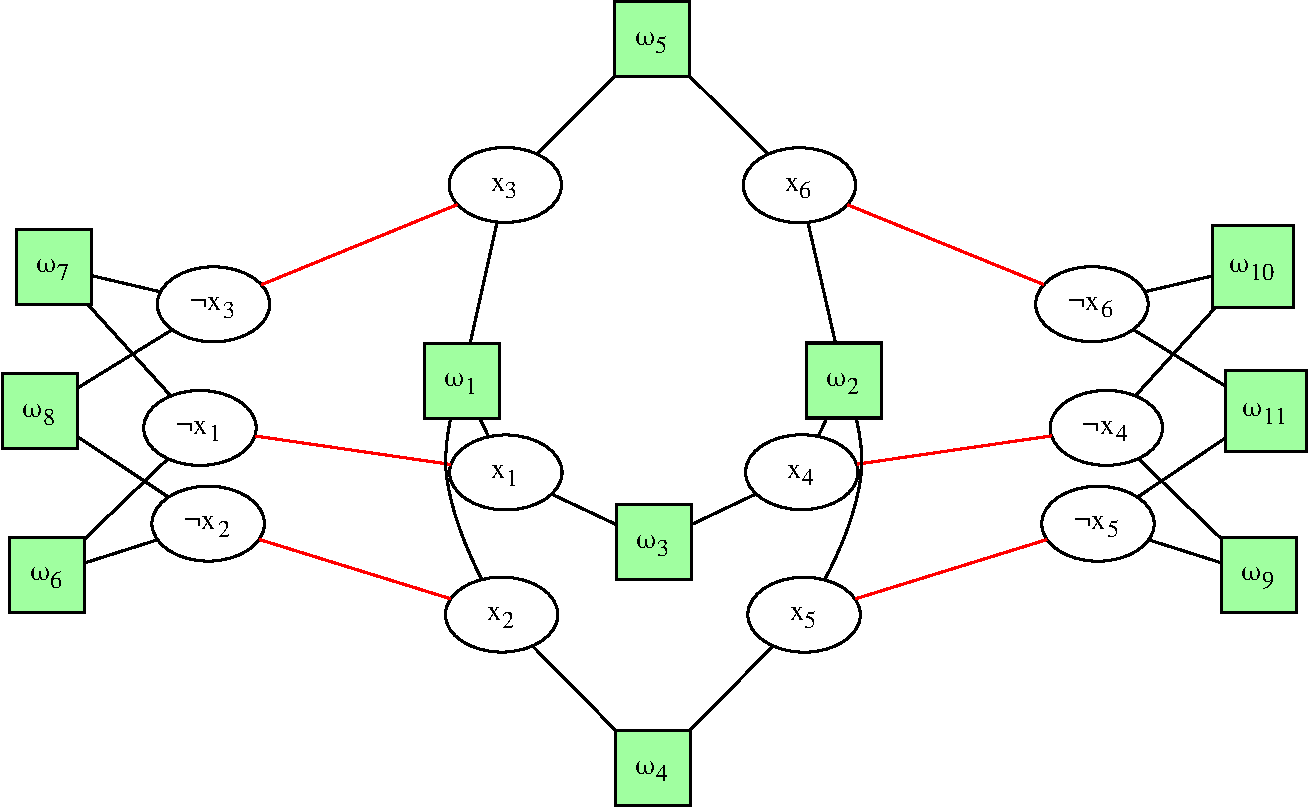
\includegraphics[width=4.3in]{cnfs/graph_cnf_no_opt-crop}
	\end{minipage}
 \caption{Example of constructed symmetry graph for a given CNF}
 \label{fig:graph_no_opt}
\end{figure}


\Cref{fig:graph_no_opt} shows the graph representation of a CNF. This problem have 6 variables and 11
clauses. So, the graph will have  12  + 11 = 33 vertexes where 12 represents literals vertexes (circle in the figure ) 
and 11 represents number of clause vertexes (square in the figure). The graph will also have 6 + 24 = 30 edges, 6 for boolean consistency 
(\hakan{XXX} color in the figure) and 24 edges that relies clauses vertexes to the literals.


% and  24 + 36 = 60 
%
%\hakan{Explication du graph + informations num nodes num edges. Probleme reel battleship
%}
%
%The battleship problems place one  ship of size *** and two ships of size* in grid 3x4 \\
%1  2  3\\
%4  5  6\\
%7  8  9\\
%10 11 12\\
%
%one ship per row.\\
%
%Produced graph contains and = 60 edges 


An optimization of this graph is possible with the usage of binary clauses i.e. a clause with only two literals.
The clause node can be omitted and we connect the two literals. As we cannot distinguish between the optimized edge 
and boolean consistency edges, we must check if the produced permutations are spurious. 
To do so, as we ensure the permutation commutes with the negation it suffice to check:
$\forall x \in \support(g), g.\neg x = \neg g.x$.
Roughly speaking, we check if the image of the negation of $x$ is equals to the negation of the image of $x$,
for each element $x$ in the support of the permutation.
This optimization allows to compute symmetries of the problem more efficiently.
In the previous example, the graph has deleted 12 nodes and 12 edges. More generally,
the graph removes as many nodes and edges as binary clauses on the formula.
\Cref{fig:graph_opt} represents the optimized version the graph.

\begin{figure}[!htbp]
	\begin{minipage}[r]{.2\textwidth}
			$\omega_{1} = \{ x_{1}, x_{2}, x_{3} \}$ \\
	$\omega_{2} = \{ x_{4}, x_{5}, x_{6} \}$ \\
	$\omega_{3} = \{ x_{1}, x_{4} \}$ \\
	$\omega_{4} = \{ x_{2}, x_{5} \}$ \\
	$\omega_{5} = \{ x_{3}, x_{6} \}$ \\
	$\omega_{6} = \{ \neg x_{1}, \neg x_{2} \}$ \\
	$\omega_{7} = \{ \neg x_{1}, \neg x_{3} \}$ \\
	$\omega_{8} = \{ \neg x_{2}, \neg x_{3} \}$ \\
	$\omega_{9} = \{ \neg x_{4}, \neg x_{5} \}$ \\
	$\omega_{10} = \{ \neg x_{4}, \neg x_{6} \}$ \\
	$\omega_{11} = \{ \neg x_{5}, \neg x_{6} \}$ \\
	\end{minipage}
	\begin{minipage}[r]{.75\textwidth}
		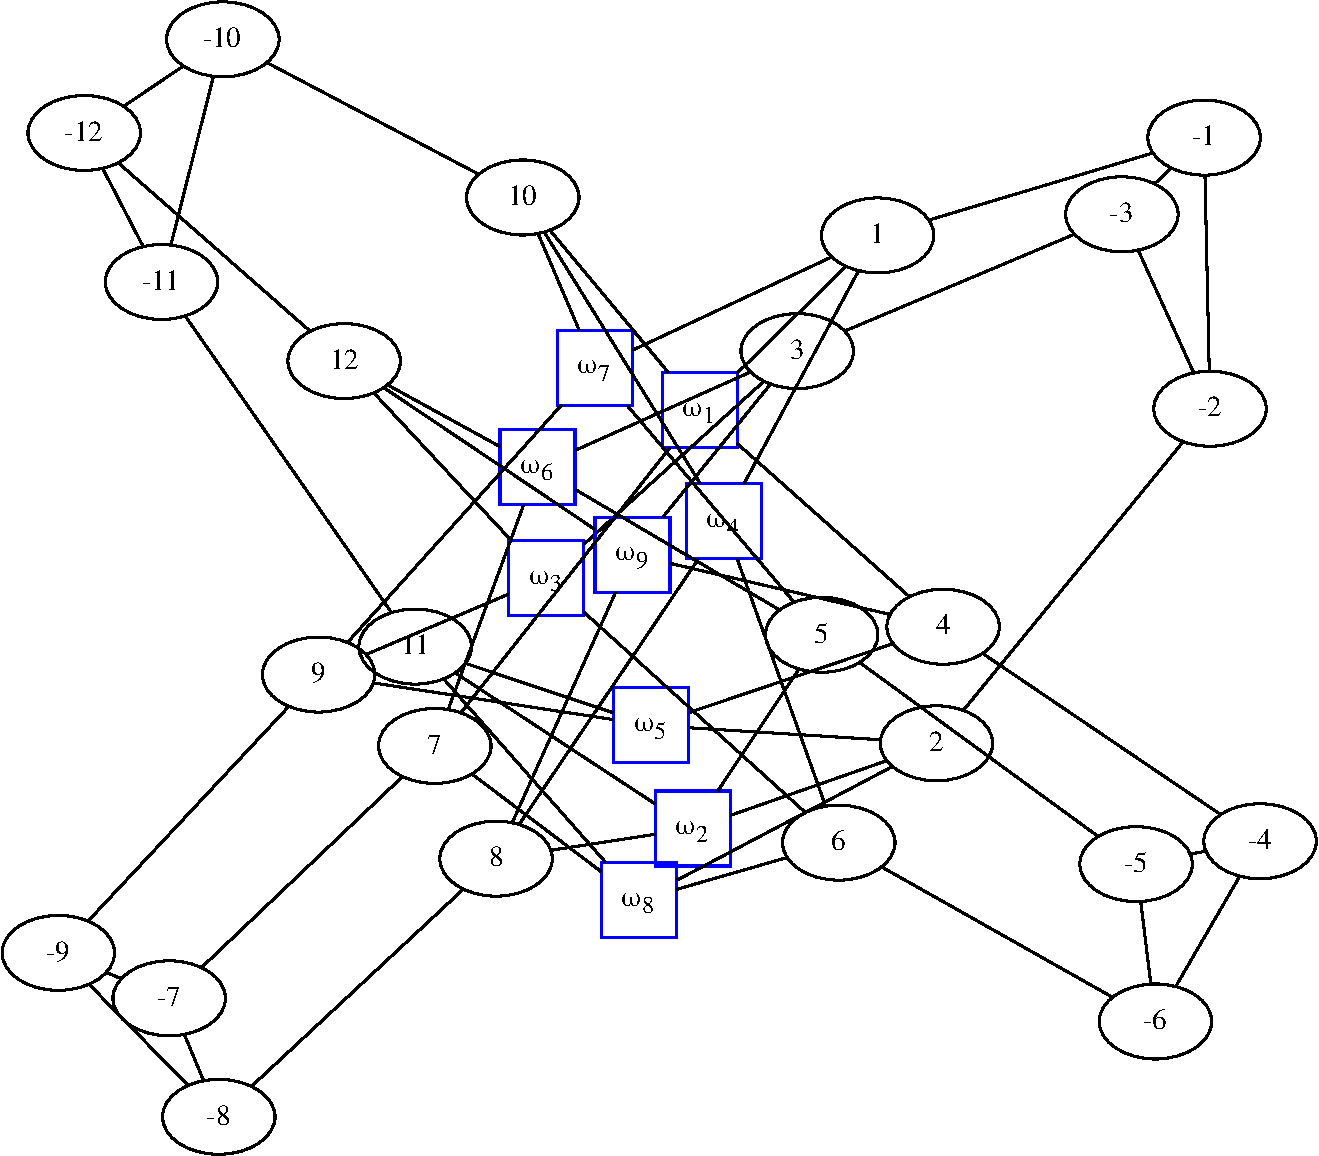
\includegraphics[width=4.3in]{cnfs/graph_cnf_opt-crop}
	\end{minipage}
	\caption{Example of constructed symmetry graph for a given CNF}
	 \label{fig:graph_opt}
\end{figure}




After the construction of a such graph, a graph automorphism tools take it as input and gives
the set of generators as output.With the previous graph, the following generators are obtained:




\begin{center}
	\begin{minipage}[c]{.635\textwidth}
		$g_1 = (x_2 \enskip x_3)(x_5 \enskip x_6)(\neg x_2 \enskip \neg x_3)(\neg x_5 \enskip \neg x_6)$\\
		$g_2 = (x_1 \enskip x_2)(x_4 \enskip x_5)(\neg x_1 \enskip \neg x_2)(\neg x_4 \enskip \neg x_5)$\\
		$g_3 = (x_1 \enskip x_4)(x_2 \enskip x_5)(x_3 \enskip x_6)(\neg x_1 \enskip \neg x_4)(\neg x_2 \enskip \neg x_5)(\neg x_3 \enskip \neg x_6)$
	\end{minipage}
\end{center}



These permutations form a permutation group and so induce an equivalence relation.
\Cref{fig:orbit} shows graphical representation of an orbit, where each node represents a literal. Two literals are linked with an arc if it exists a permutation that maps one to the other. 
An orbit must be a \emph{strongly connected component} (SCC).  
Some permutations have a special form like two dimensional
array as in this example.
 A further section (\ref{sec:matrix-sbp}) shows how to exploit this special form.

\begin{figure}[!htbp]
	

\begin{center}
	

\begin{tikzpicture}
	\tikzstyle{orbit-node}=[draw,circle,minimum size=35pt,inner sep=0pt]
	\tikzstyle{g1}=[->, draw, color=blue_1, line width=1pt]
	\tikzstyle{g2}=[->, draw, color=green_1, line width=1pt]
	\tikzstyle{g3}=[->, draw, color=red_1, line width=1pt]
	
	\node[orbit-node] (1) {$x_1$};
	\node[orbit-node] (2) at ($(1) + (5, 0)$) {$x_2$};
	\node[orbit-node] (3) at ($(2) + (5, 0)$) {$x_3$};
	\node[orbit-node] (4) at ($(1) + (0, -4)$) {$x_4$};
	\node[orbit-node] (5) at ($(1) + (5, -4)$) {$x_5$};
	\node[orbit-node] (6) at ($(2) + (5, -4)$) {$x_6$};
	
	% g1
	\draw[g1] (1) to [bend right=10] (2);
	\draw[g1] (2) to [bend right=10] (1);
	
	\draw[g1] (4) to [bend right=10] (5);
	\draw[g1] (5) to [bend right=10] (4);
	
	
	%g2
	
	\draw[g2] (2) to [bend right=10] (3);
	\draw[g2] (3) to [bend right=10] (2);
	
	\draw[g2] (5) to [bend right=10] (6);
	\draw[g2] (6) to [bend right=10] (5);
	
	% g3
	\draw[g3] (1) to [bend right=10] (4);
	\draw[g3] (4) to [bend right=10] (1);
	
	\draw[g3] (2) to [bend right=10] (5);
	\draw[g3] (5) to [bend right=10] (2);
	
	\draw[g3] (3) to [bend right=10] (6);
	\draw[g3] (6) to [bend right=10] (3);
	
\end{tikzpicture}

\end{center}
	\caption{Graphical representation of an orbit}
	\label{fig:orbit}
\end{figure}



\section{Usage of symmetries}

\emph{Symmetry breaking} aims at eliminating symmetry, either
by \emph{statically} posting symmetry breaking constraints that invalidate symmetric
assignments, or by altering the search space \emph{dynamically} to avoid symmetric search paths.


\subsection{Static symmetry breaking}

One way to exploit symmetry properties is to forbid equivalent assignments except one.
Let introduce an ordering relation between the assignments.

\begin{definition}[Assignments ordering]
	\label{def:assignment_ordering}
	We assume a total order, $\prec$, on $\Vars$.  Given two assignments $(\alpha,\beta) \in \Assignments(\Vars)^2 $, 
	we say that $\alpha$ is strictly smaller than $\beta$, noted $\alpha < \beta$, if there exists a variable $v \in \Vars$
	such that:
	\begin{itemize}
		\item for all $v' \prec v$, either $v' \in \alpha \cap \beta$ or $\neg v' \in \alpha \cap
		\beta$.
		\item $\neg v \in \alpha$ and $v \in \beta$ \footnote{We could have chosen as well 
			$v \in \alpha$ and $\neg v \in \beta$ without loss of generality.}.
	\end{itemize}
\end{definition}


In other word, the prefix of both assignment are equals according to the ordering relation~$\prec$
and the next variable $v$ has a different value, $\alpha(v) = \false, \beta(v) = \true$, then $\alpha < \beta$.
Note that $<$ coincides with the lexicographical order on \emph{complete}
assignments. 

Furthermore, the $<$ relation is monotonic as expressed in the following proposition:

\begin{proposition}[Monotonicity of assignments ordering]
	\label{prop:monocity_assignments_ordering}
	Let  $(\alpha,\alpha',\beta,\beta') \in \Assignments(\Vars)^4 $ be four assignments.
	$$\text{If}~\alpha \subseteq \alpha'~\text{and}~\beta \subseteq \beta',~\text{then}~\alpha < \beta \implies \alpha' < \beta'$$
\end{proposition}

\begin{proof}
	The proposition follows on directly from Definition \ref{def:assignment_ordering}.
\end{proof}


Given a formula $\varphi$ and its group of symmetry $G$,
the \emph{orbit of $\alpha$ under $G$} (or
simply the \emph{orbit of $\alpha$} when $G$ is clear from the context) is the set
$ [\alpha]_G=\{ g.\alpha \mid g \in G \}$. 
The lexicographic leader (\textit{lex-leader} for short) of an orbit $[\alpha]_G$ is defined by
$min_<([\alpha]_G)$. This \textit{lex-leader} is unique because the lexicographic
order is a total order.
The optimal approach to solve a symmetric SAT problem would be to explore
only one assignment per orbit (for instance each lex-leader). \Cref{fig:lex-leader} shows different orbits, each dot in an orbit (ellipse in the figure) is an assignment, and the lex-leader is the empty red one.
To avoid exploring 
symmetry search space, \emph{symmetry breaking predicates} (SBP) also called \emph{lex-leader constraints} 
are added to the formula.
These constraints are only true for the \emph{lex-leader} \cite{crawford1996symmetry} and prevents other assignments from being explored. 

\begin{figure}[!htbp]
	\centering
	%	\includegraphics[width=2in]{fig/assignment-lex-leader}
	\begin{tikzpicture}
    \tikzstyle{point}=[circle,draw,thick,fill=black,scale=0.2]
	\tikzstyle{point+}=[circle,draw=red,thick,scale=0.4]


\begin{scope}
\node[ellipse, draw, minimum width=4cm, minimum height=2cm] (c1) at (2.5,0){};
	\clip (2.5, 0) ellipse (2 and 1);
	\node[point+] (p2) at (1, 0.3){};
	\pgfmathsetseed{281}
	\foreach \p in {1,...,100}
	{
		\fill (4*rand,2*rand+0.25) circle (0.08);
	}
\end{scope}


\begin{scope}
\node[ellipse, draw, minimum width=4cm, minimum height=2cm] (c1) at (8.5,0){};
\clip (8.5,0) ellipse (2 and 1);
\node[point+] (p2) at (8.6, -0.1){};
\pgfmathsetseed{499478626}
\foreach \p in {1,...,40}
{
	\fill (4*rand+6,2*rand) circle (0.08);
}
\end{scope}

% Legend

\path[draw] (-1, -1.5) -- (13, -1.5);
\node[draw,ellipse, draw, minimum width=4cm, minimum height=2cm, scale=0.1] (ld) at (0, -2) {};
\node[align=left, text width=2.2cm] at (1.5, -2) {Orbit};


\node[circle, fill=black, draw=black, line width=0.5mm, scale=0.3] (lz) at (3, -2) {};
\node[align=left, text width=2.2cm] at (4.5, -2) {Assignment};


\node[point+] (le) at (7, -2) {};
\node[align=left, text width=4.2cm] at (9.5, -2) {Lex-leader assignment};

\path[draw] (-1, -2.7) -- (13, -2.7);



\end{tikzpicture}
	\caption{Show lex-leader per orbit}
	\label{fig:lex-leader}
\end{figure}


Lex-leader predicates for a permutation $g \in G_\varphi$ is defined as :
$$LL_g = \forall i : (\forall j < i : x_j = g.x_j) \Rightarrow  x_i \preceq g.x_i$$

In other words, each assignment whose have a variable such that its image under $g$ is smaller according to the ordering relation $\prec$, is pruned by $LL_g$.
Conjunction of $LL_g$, for all permutation  $g \in G_{\varphi} $ results a sound and complete symmetry breaking predicates also called \emph{full symmetry breaking}. Only lex-leader assignment will be visited 
per orbit. Hence, finding the lex-leader of an orbit is computationally hard~\cite{Luks2004}. 
Conjunction of $LL_g$ for some $G \subset G_{\varphi}$ results a symmetry breaking predicates that aims to
visit at least one assignment per orbit and called is \emph{partial symmetry breaking}.
In both case, the set of symmetry breaking predicates generated is denoted as $\psi$.

Since  a group may have a exponential number of permutations, all symmetry breaking predicates belongs
to the group must be generated to ensure full symmetry breaking. These constraints will overload the 
solver and slow down its core (unit propagation). Hence, slow down overall time computation.
Conversely, partial symmetry breaking add few constraints and bring often considerable reduction of the
search space. Generally, the set of generators produced by automorphism tool is chose as subgroup.
Partial symmetry breaking gives a good trade off between number of generated constraints and reduction of the search space.


%
%To ensure the visiting only the lex leader, all SBPs of all permutations 
%belongs to the group must be generated.
%Adding too many SBPs clauses will overload the solver and slow down the unit propagation.
%
%When only one assignment per orbit (generally the lex-leader) is visited, this is called  \emph{full symmetry breaking}.
%Conversely, \emph{partial symmetry breaking} aims to visit at least one assignment per orbit.
%Only some of the permutations are used to generate SBPS, that are generally  the set of generators 
%given by the automorphism tool.
%This approach is more easy to set up and bring considerable reduction of the search spaces.

%in some $G \subseteq G_{\varphi} $ results a sound and complete symmetry breaking predicates
%but not necessarily \emph{complete} symmetry breaking predicates for $G_{\varphi}$ noted $\psi$.



\begin{theorem}[Satisfiability preservation SBPs]
	\label{theorem:satisfiability_preservation_SBPs}
	Let $\varphi$ be a formula and $\psi$ the computed \textit{SBPs} for the set of	symmetries in $G_{\varphi}$:
	
	$$\varphi~and ~\varphi \wedge \psi \text{ are equi-satisfiable}.$$
\end{theorem}

\begin{proof}
	If $\varphi \wedge \psi$ is SAT then $\varphi$ is trivially SAT. If
	$\varphi$ is SAT, then there is some assignment $\beta$ that satisfies $\varphi$.
	Without loss of generality, $\beta$ can be chosen to be the lex-leader of its
	orbit under $G_{\varphi}$. Thus, $g$ does not contradict $\beta$, which implies that
	$\beta \models \psi$.
\end{proof}




% By definition of an orbit, it exists a permutation that map each assignment to another in the same orbit. 


%
%Lex-leader constraints are build for each permutation in the group.
%Given a permutation 
%Generation of these lex-leaders constraints proposed by Crawford et al.~\cite{crawford1996symmetry}:
%
%$$\forall i : (\forall j < i : x_j = g.x_j) \Rightarrow  x_i \preceq g.x_i$$
%
%In other words, assuming the ordering relation depicted in \Cref{def:assignment_ordering}, for one permutation,
%these constraint express that the value of the variable $x_i$ must be smaller or equal than the
%value of $g.x_i$ and all variables $x_j$ that respect the constraint $x_j \prec x_i$,  
%must have the same value of its symmetric. As such, these constraints encodes a valid 
%lex leader with respect to this permutation.


Generation of lex-leader constraints proposed by Crawford et al.~\cite{crawford1996symmetry} is defined as follow:
$$ LL_g = \forall i : (\forall j < i : x_j = g.x_j) \Rightarrow  \neg x_i \lor g.x_i$$

 
 \Cref{fig:esbp_gen} shows an example of generated clauses for the  permutation $g_3$ of the previous 
 example and an lexicographic order. Last constraint present in the figure produce tautological clause,
 effectively variable $x_1$ or $x_4$ are present in both polarity. The constraints of other variables produce 
 also tautological clauses. 
 
 
 \begin{figure}[!htbp]
 	
total order $ x_1 \prec x_2 \prec x_3 \prec x_4 \prec x_5 \prec x_6$\\
permutation $g_1 = (x_2 \enskip x_3)(x_5 \enskip x_6)(\neg x_2 \enskip \neg x_3)(\neg x_5 \enskip \neg x_6)$\\


$x_2 \preceq x_3$ \\
$x_2 = x_3 \implies x_5 \preceq x_6$\\

%2 == 3 -> 3 <= 2
%2 == 3 \land 3 == 2 -> 5 <= 6
 	\caption{Example of generated SBPs for one permutation}
 	\label{fig:esbp_gen}
 \end{figure}
 
 
 Moreover, the number of clauses generated per constraint increase exponentially with the number of variable present in the permutation.
  Hence, Aloul et al~\cite{aloul06} propose a more compact representation of  symmetry breaking predicates.
 
 Let $g$ a permutation, let $\support_g$ = $\{x_1, \cdots, x_n\}$ the support of the permutation $g$ be ordered 
 such that $x_i \preceq x_j$ iff $i \leq j$  and let $\{y_0,\cdots, y_{n} \}$ be a set of auxiliary variables
 disjoint from $\support_g$. These auxiliary variables encode equality of literals in such $y_0$ is set as an unit clause
 and encode the first equality.
 Following clauses encode a compact lex-leader for a permutation:
 

\begin{center}
\begin{tabular}{cc|cc}
	$\neg y_i \lor \neg x_{i-1} \lor \neg x_i \lor g.x_i$ & $1 \leq i \leq n$ & $ \neg y_i \lor \neg x_{i-1} \lor \neg y_{i+1}$ & $1 \leq i \leq n$ \\
	$\neg y_i \lor  g.x_{i-1} \lor \neg x_i \lor g.x_i$ & $1 \leq i \leq n$ & $ \neg y_i \lor g.x_{i-1} \lor \neg y_{i+1}$ & $1 \leq i \leq n$ \\
	
\end{tabular}
\end{center}



\Cref{fig:esbp_compact_gen} shows the compact encoding of generated clauses. This form grow linearly with the number of variables.
Auxiliary variable encodes the equality of two literals allows to achieve this reduction. Three auxiliary variables are introduced
in this example $x_7, x_8, x_9$ such that $x_7$ encode the equality of $x_1$ and $x_4$, $x_8$ equality of $x_2$ and $x_5$, and $x_9$ equality of $x_3$ and $x_6$.

 \begin{figure}[!htbp]
	


\begin{center}
	\begin{tabular}{lll}
		Order &:& $ x_1 \prec x_2 \prec x_3 \prec x_4 \prec x_5 \prec x_6 \enskip ; \enskip  (\false < \true)$ \\
		Permutation &:& $g_3 = (x_1 \enskip x_4)(x_2 \enskip x_5)(x_3 \enskip x_6)(\neg x_1 \enskip \neg x_4)(\neg x_2 \enskip \neg x_5)(\neg x_3 \enskip \neg x_6)$
	\end{tabular}
	
	\vspace*{2\baselineskip}
	
	\begin{tabular}{ll}
		Constraints & Generated SBP\\
		\midrule
		$x_1 \preceq x_4$ & $ \neg x_1 \lor x_4$ \\
		& $x_7$ \\
		&\\
		$x_1 = x_4 \Rightarrow x_2 \preceq x_5$ &  $ \neg x_7 \lor \neg x_1 \lor \neg x_2 \lor x_5$\\
		& $ \neg x_7 \lor \neg x_1 \lor x_8$\\
		& $ \neg x_7 \lor  x_4 \lor \neg x_2 \lor x_5$ \\
		& $ \neg x_7 \lor x_4 \lor x_8$\\
		
		&\\
		$x_1 = x_4 \land x_2 = x_5 \Rightarrow x_3 \preceq x_6$ 
		& $\neg x_8 \lor \neg x_2 \lor \neg x_3 \lor x_6$\\
		& $\neg x_8 \lor \neg x_2 \lor x_9$\\
		& $\neg x_8 \lor x_5 \lor \neg x_3 \lor x_6$\\
		& $\neg x_8 \lor x_5 \lor x_9$\\

	\end{tabular}
\end{center}
	\caption{Example of compact generated SBPs for one permutation}
	\label{fig:esbp_compact_gen}
\end{figure}


\shatter~\cite{aloul06} is a tool fot partial symmetry breaking that computes symmetry with $\saucy$ automorphism tool and generate a new formula with compact lex-leader encoding. It uses only generators given by the automorphism tool. Following table shows the number of symmetry breaking predicates clauses and the
number of auxiliary variables added to the original formula.



\begin{center}
	\hakan{Mette des espaces pour les nombres et texte pour expliquer si tableau ok}\\
	\hakan{Mettre total de clause et vars et pourcentage d'augmentation}
\begin{tabular}{lcccc}
	Instances & \#vars & \#clause & \#sbp & \#auxiliary variables \\
	\toprule
	\detokenize{battleship-12-12-unsat} &  936 &  144 &  1498 &  378\\
	\detokenize{battleship-12-23-sat} &  1662 &  276 &  5464 &  1375\\
	\detokenize{battleship-14-26-sat} &  2562 &  364 &  3688 &  929\\
	\detokenize{battleship-14-27-sat} &  2653 &  378 &  7222 &  1814\\
	\detokenize{battleship-16-16-unsat} &  2176 &  256 &  4388 &  1102\\
	\detokenize{battleship-16-31-sat} &  3976 &  496 &  12094 &  3035\\
	\detokenize{battleship-24-57-sat} &  16308 &  1368 &  40372 &  10113\\
	\midrule
	\detokenize{chnl10_11} &  1122 &  220 &  2416 &  615\\
	\detokenize{chnl10_12} &  1344 &  240 &  2736 &  696\\
	\detokenize{chnl10_13} &  1586 &  260 &  3252 &  826\\
	\detokenize{chnl11_12} &  1476 &  264 &  3204 &  813\\
	\detokenize{chnl11_13} &  1742 &  286 &  3636 &  922\\
	\detokenize{chnl11_20} &  4220 &  440 &  6760 &  1710\\
	\midrule
	\detokenize{fpga10_15_uns_rcr} &  2130 &  300 &  4580 &  1160\\
	\detokenize{fpga10_20_uns_rcr} &  3840 &  400 &  6768 &  1712\\
	\detokenize{fpga11_12_uns_rcr} &  1476 &  264 &  3704 &  938\\
	\detokenize{fpga11_13_uns_rcr} &  1742 &  286 &  4076 &  1032\\
	\detokenize{fpga11_14_uns_rcr} &  2030 &  308 &  4740 &  1199\\
	\detokenize{fpga11_15_uns_rcr} &  2340 &  330 &  5196 &  1314\\
	\detokenize{fpga11_20_uns_rcr} &  4220 &  440 &  7864 &  1986\\
	\midrule
	\detokenize{hole010} &  561 &  110 &  1054 &  269\\
	\detokenize{hole015} &  1816 &  240 &  3280 &  828\\
	\detokenize{hole020} &  4221 &  420 &  6478 &  1630\\
	\detokenize{hole030} &  13981 &  930 &  21322 &  5346\\
	\detokenize{hole040} &  32841 &  1640 &  44934 &  11254\\
	\detokenize{hole050} &  63801 &  2550 &  81682 &  20446\\
	\midrule
	\detokenize{Urq6_5} &  1756 &  180 &  109 &  0\\
	\detokenize{Urq7_5} &  2194 &  240 &  143 &  0\\
	\detokenize{Urq8_5} &  3252 &  327 &  200 &  0\\
	\midrule
	\detokenize{x1_40} &  314 &  118 &  42 &  1\\
	\detokenize{x1_80} &  634 &  238 &  80 &  0\\
\end{tabular}
\end{center}



%\hakan{mettre tableauw nombre de SBP generé}
%
%\begin{figure}[!htbp]
%	\centering
%	\includegraphics[height=5cm]{example-image-a}
%	\label{}
%\end{figure}



An improvement of static symmetry breaking was made by Devriendt et al~\cite{devriendt2016improved} with a tool 
called $\breakid$. It exploits some properties from the structure of generators. On some circumstance 
a linear number of constraints can break all group. The other tries to add a maximum of binary clauses that 
is useful because it can participate often to unit propagation and so to the conflict analysis.


\subsubsection{Special form of the group} \label{sec:matrix-sbp}
Some formula presents specific type of symmetry called \emph{row (column) interchangeability}, when a
subset of variables are structured as a two dimensional matrix. Each row (column) are interchangeable
with the symmetries. 
This form of symmetry is common in different kind of problem like pigeon hole problem in which
pigeons and holes are interchangeable or in delivery system in which trucks of a fleet are interchangeable.
Usage of row (column) interchangeability can significantly improved SAT performance. 
Effectively symmetries can be eliminated by the addition 
of only a linear number of symmetry-breaking constraints~\cite{flener2002breaking}. 
One condition must be satisfied to ensure this linear number of constraints:
lexicographic order needs to respect the structure of the matrix.
In practice, automorphism tools gives only the set generators which contains no information on
the structure of the group. 
Authors of $\breakid$~\cite{devriendt2016improved} develop an algorithm to detect this specific 
structure and exploit it.



\subsubsection{Binary leax-leader constraints}

$\breakid$ has another approach that aims to post many lex-leader constraints.
The first constraint of symmetry breaking predicates must produce a binary clause.
Building many binary clauses is possible without enumerating the whole symmetry group. 
It suffices to compute the orbit of the smallest variable according to the ordering relation. As the orbit can be seen as a strong connected component, it must exist a permutation that permutes the smallest variable with all other variables in the same orbit.
Then, as many binary clauses as variables (without the smallest variable) in the orbit can be added to the formula. Constructing a sequence of subgroups that stabilize the smallest variable (i.e. not have the smallest variable in its support) results to new binary clauses.
This sequence ends when trivial subgroup is reached and is called a  \emph{stabilizer chain}.


\Cref{fig:binary_sbp} shows application of the generation of binary clauses.
In the example, considered group has three permutations and its graphical representation
is show. Given the lexicographic order, the smallest variable is $x_1$ and 
all other variables are in its orbits. According to the ordering relation, five 
symmetry breaking predicates are generated with the formula $\neg x_1 \lor g.x_1$.
Then, subgroup that stabilize $x_1$ is computed and it remains only one permutation $g_2$.
As it smallest variable is $x_2$, the constraint $\neg x_2 \lor x_3$ is generated.
Stabilizer chain leads to trivial group and no more binary clauses are generated.

In total, six binary clauses is generated without adding any auxiliary variables.
Moreover, a property can be observed, when the smallest variable have the greatest value 
(\true in this case), all variables in the orbits must have the same value.

 \begin{figure}[!htbp]
	
\begin{center}
\begin{tabular}{lll}
	Order &:& $ x_1 \prec x_2 \prec x_3 \prec x_4 \prec x_5 \prec x_6 \enskip \mid \enskip  (\false < \true)$ \\
\end{tabular}
\end{center}
\vspace*{1\baselineskip}
	
\begin{minipage}[c]{.635\textwidth}
	\footnotesize
	$\textcolor{green_1}{g_1 = (x_2 \enskip x_3)(x_5 \enskip x_6)(\neg x_2 \enskip \neg x_3)(\neg x_5 \enskip \neg x_6)}$\\
	$\textcolor{blue_1}{g_2 = (x_1 \enskip x_2)(x_4 \enskip x_5)(\neg x_1 \enskip \neg x_2)(\neg x_4 \enskip \neg x_5)}$\\
	$\textcolor{red_1}{g_3 = (x_1 \enskip x_4)(x_2 \enskip x_5)(x_3 \enskip x_6)(\neg x_1 \enskip \neg x_4)(\neg x_2 \enskip \neg x_5)(\neg x_3 \enskip \neg x_6)}$

	\vspace*{2\baselineskip}
	
\begin{tikzpicture}[level/.style={sibling distance=60mm/#1},every node/.style={scale=0.6}, scale=0.6]
	\tikzstyle{orbit-node}=[draw,circle,minimum size=35pt,inner sep=0pt]
	\tikzstyle{g1}=[->, draw, color=blue_1, line width=1pt]
	\tikzstyle{g2}=[->, draw, color=green_1, line width=1pt]
	\tikzstyle{g3}=[->, draw, color=red_1, line width=1pt]
	
	\tikzstyle{g}=[->, draw, color=black, line width=1pt]
		
	\node[orbit-node, fill=orange!30] (1) {$x_1$};
	\node[orbit-node] (2) at ($(1) + (5, 0)$) {$x_2$};
	\node[orbit-node] (3) at ($(2) + (5, 0)$) {$x_3$};
	\node[orbit-node] (4) at ($(1) + (0, -4)$) {$x_4$};
	\node[orbit-node] (5) at ($(1) + (5, -4)$) {$x_5$};
	\node[orbit-node] (6) at ($(2) + (5, -4)$) {$x_6$};
	
	% g1
	\draw[g1] (1) to [bend right=10] (2);
	\draw[g1] (2) to [bend right=10] (1);
	
	\draw[g1] (4) to [bend right=10] (5);
	\draw[g1] (5) to [bend right=10] (4);
	
	
	%g2
	
	\draw[g2] (2) to [bend right=10] (3);
	\draw[g2] (3) to [bend right=10] (2);
	
	\draw[g2] (5) to [bend right=10] (6);
	\draw[g2] (6) to [bend right=10] (5);
	
	% g3
	\draw[g3] (1) to [bend right=10] (4);
	\draw[g3] (4) to [bend right=10] (1);
	
	\draw[g3] (2) to [bend right=10] (5);
	\draw[g3] (5) to [bend right=10] (2);
	
	\draw[g3] (3) to [bend right=10] (6);
	\draw[g3] (6) to [bend right=10] (3);
	
	\draw[g] (1) to [bend left=25] (3);
	\draw[g] (1) to [] (5);
	\draw[g] (1) to [bend left=0] (6);
\end{tikzpicture}
\end{minipage}
\begin{minipage}[c]{.635\textwidth}
	\footnotesize
	$\textcolor{green_1}{g_1 = (x_2 \enskip x_3)(x_5 \enskip x_6)(\neg x_2 \enskip \neg x_3)(\neg x_5 \enskip \neg x_6)}$\\
	
	\vspace*{4.5\baselineskip}
	
	\begin{tikzpicture}[level/.style={sibling distance=60mm/#1},every node/.style={scale=0.6}, scale=0.6]
	\tikzstyle{orbit-node}=[draw,circle,minimum size=35pt,inner sep=0pt]
	\tikzstyle{g1}=[->, draw, color=blue_1, line width=1pt]
	\tikzstyle{g2}=[->, draw, color=green_1, line width=1pt]
	\tikzstyle{g3}=[->, draw, color=red_1, line width=1pt]
	
	\tikzstyle{g}=[->, draw, color=black, line width=1pt]
	
	\node[orbit-node,fill=orange!30] (2) {$x_2$};
	\node[orbit-node] (3) at ($(1) + (5, 0)$) {$x_3$};

	\node[orbit-node] (5) at ($(1) + (0, -4)$) {$x_5$};
	\node[orbit-node] (6) at ($(1) + (5, -4)$) {$x_6$};

	\draw[g2] (2) to [bend right=10] (3);
	\draw[g2] (3) to [bend right=10] (2);
	
	\draw[g2] (5) to [bend right=10] (6);
	\draw[g2] (6) to [bend right=10] (5);
	
	\end{tikzpicture}
\end{minipage}

\vspace*{1\baselineskip}

\begin{minipage}[l]{.58\textwidth}
	\begin{itemize}
		\item[] $\omega_{1} = \{\neg x_1, x_2\}$\hspace*{2em} $\omega_{4} = \{\neg x_1, x_5\}$
		\item[] $\omega_{2} = \{\neg x_1, x_3\}$\hspace*{2em} $\omega_{5} = \{\neg x_1, x_6\}$
		\item[] $\omega_{3} = \{\neg x_1, x_4\}$
	\end{itemize}
\end{minipage}
\begin{minipage}[l]{.635\textwidth}
	\begin{itemize}
		\item[] $\omega_{6} = \{\neg x_2, x_3\}$
	\end{itemize}
\end{minipage}
	\caption{Caption}
	\label{fig:binary_sbp}
\end{figure}


The size of the stabilizer chain is heavily dependent of the chose lexicographic order.
More stabilizer discard permutations and more trivial subgroup is reached quickly and less 
binary clauses are generated. An incremental order is proposed to optimize number of generates binary clauses. First, orbit of all variables is computed and the variable with fewest number of occurrence is chose among the biggest orbit. The idea is that biggest orbit produce more
clauses and the variable appearing in few permutations reduce the number of stabilized permutation. This procedure is applied until trivial group is reached. At the end, remaining variables are added to the order.



\subsection{Evaluation of performance}



\hakan{Faire une section pour ça}
An extremely important point is the chosen lexicographic order.
Variable ordering may impact the number of generated constraint and so the performance of
the underlying SAT solver. Different orders are studied in the literature. 
One of the simplest order was the sorted variables according to their numbers.
Some others orders exists and exploit structural properties of the 
problem. In particular, the orbits of the variables in different ways. For example, the variables are chosen 
with their number of occurrences in the initial problem. This order, is equivalent to put largest orbit first
and so on, because each variable on the same orbit must have the same number of occurrences.
Another example of exploiting structural property of the orbit is the usage of \emph{stabilizer}.
The order choose a variable which maximize the number of stabilized permutations, removes the not stabilized ones and loop over until the empty set. The remaining variables are added to the order to get a complete order.



%The exploitation of symmetries statically is called \emph{static symmetry breaking}.
%It acts like a preprocessor which add \emph{symmetry breaking predicates} (SBPs) at the 
%original formula and solve the augmented problem. 
%This approach gives good performances in practice.
%
%\hakan{Generation des clauses de SBPs}\\
%\hakan{Parler des groupes speciaux  (totaux) }\\
%\hakan{Generation des clause binaires breakid lie aux orbits}\\
%\hakan{Parler de BreakID all in one tout au dessus}\\
%
%\hakan{Put a complete exemple}\\
%
%\hakan{Mettre des courbes}\\
%\hakan{Tableau sur le nombre de sbp genere}\\
%
%\hakan{ Shatter, BreakID}
%
%\hakan{Conclu static}




\subsubsection{Conclusion}

Static symmetry breaking acts as a preprocessor that augment the initial formula with
symmetry breaking predicates. These constraints avoid exploration of symmetric search space.
In the general case, the number of these clauses are often too large to be
effectively handled by a SAT solver~\cite{Luks2004}. 
On the other hand, if only a subset of the symmetries is considered then the resulting search pruning
will not be perfect and its effectiveness depends heavily on the
heuristically chosen symmetries \cite{biere2009handbook}.
\hakan{Parler des optim de BReakID}
Despite the good reduction of the search space, some formula still intractable for a 
state of the art SAT solver.


%\begin{figure}[!htbp]
%	  \newcolumntype{C}{ >{\centering\arraybackslash} m{8cm} }
  \newcolumntype{D}{ >{\centering\arraybackslash} m{6cm} }
  \begin{tabular}{DC}
    CNF\ formula &{\scriptsize
          \begin{tabular}{c}
          	$ \{ x_{1}, x_{2}, x_{3} \}$,
          	$ \{ x_{4}, x_{5}, x_{6} \}$,
          	$ \{ x_{1}, x_{4} \}$ \\
          	$ \{ x_{2}, x_{5} \}$,
          	$ \{ x_{3}, x_{6} \}$ ,
          	$ \{ \neg x_{1}, \neg x_{2} \}$ \\
          	$ \{ \neg x_{1}, \neg x_{3} \}$,
          	$ \{ \neg x_{2}, \neg x_{3} \}$,
          	$ \{ \neg x_{4}, \neg x_{5} \}$\\
          	$ \{ \neg x_{4}, \neg x_{6} \}$,
          	$ \{ \neg x_{5}, \neg x_{6} \}$            
          \end{tabular}}\\
      & \\
    $\Downarrow$ & $\Downarrow$  \\
          & \\
    colored graph & 		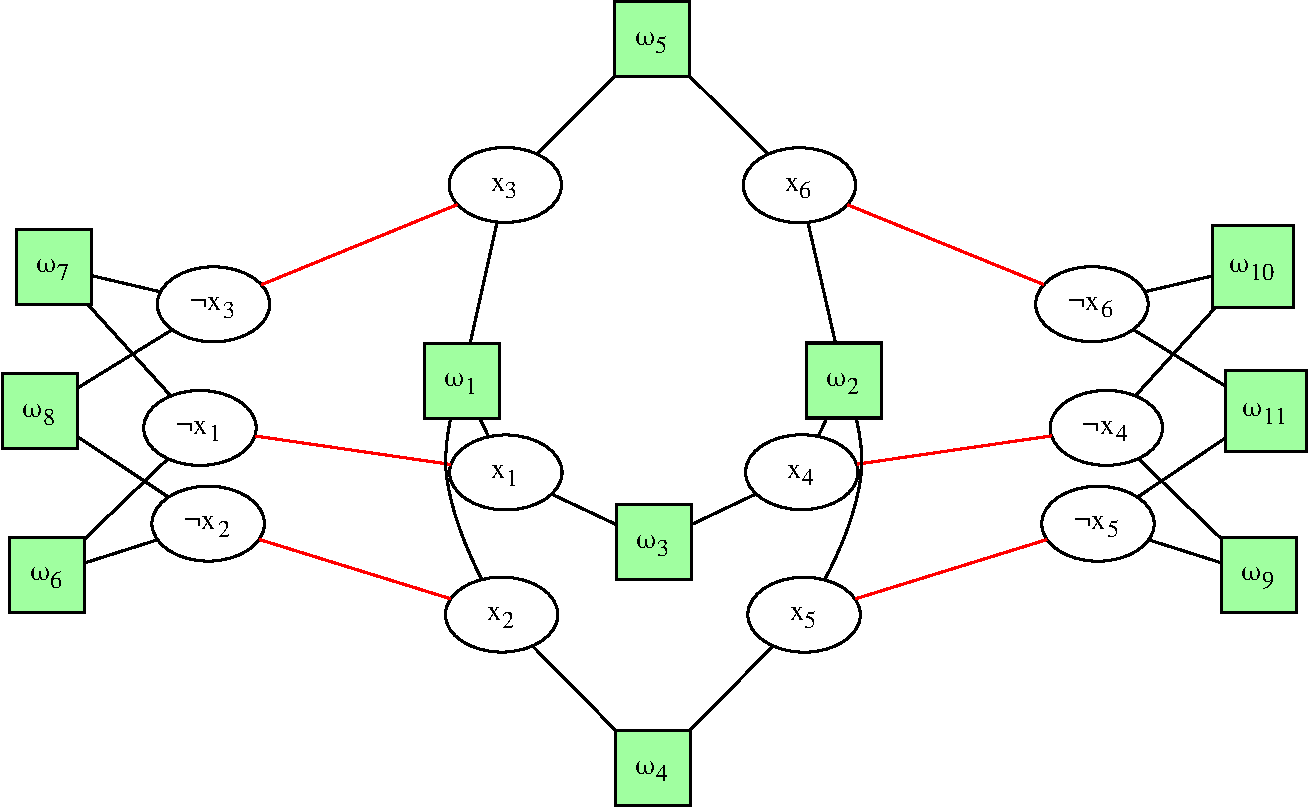
\includegraphics[width=2.5in]{cnfs/graph_cnf_no_opt-crop}\\

    $\|$ & $\|$  \\
        & \\
    graph automorphism &
                         \small{(\texttt{bliss} \footnote{http://www.tcs.hut.fi/Software/bliss/} or
                         \texttt{saucy} \footnote{http://vlsicad.eecs.umich.edu/BK/SAUCY/})}
    \\
  
        & \\
    $\Downarrow$ & $\Downarrow$  \\
      & \\
    set of symmetries & \begin{minipage}[l]{\textheight}
    	\footnotesize
    	$g_1 = (x_2 \enskip x_3)(x_5 \enskip x_6)(\neg x_2 \enskip \neg x_3)(\neg x_5 \enskip \neg x_6)$\\
    	$g_2 = (x_1 \enskip x_2)(x_4 \enskip x_5)(\neg x_1 \enskip \neg x_2)(\neg x_4 \enskip \neg x_5)$\\
    	$g_3 = (x_1 \enskip x_4)(x_2 \enskip x_5)(x_3 \enskip x_6)(\neg x_1 \enskip \neg x_4)(\neg x_2 \enskip \neg x_5)(\neg x_3 \enskip \neg x_6)$
    \end{minipage}  \\
  \end{tabular}
%	\caption{Caption}
%	\label{fig:big_picture_static}
%\end{figure}




\subsection{Dynamic symmetry breaking}


Another disadvantage is that the solver is influenced by SBPs and explore the search space with a different 
manner and can affect performance negatively \hakan{FIND A REF}

In the literature, different approach of dynamic symmetry breaking are used to reduce the search space
of the sat solver in different ways. Some of them \textit{inject} constraints to allow only one representative assignment of each orbit like the static approach and others accelerate the propagation of variable using symmetrical properties. In this section, we present different approach to use symmetrical properties of a problem 
dynamically.


\subsubsection{SymChaff}

One of the first dynamic symmetry breaking approach is \emph{SymChaff}~\cite{sabharwal2005symchaff}
and is applicable only on special groups where all couple of variables are symmetric.
The idea of this approach is to treat each orbit like a \emph{symbolic variable}, i.e. instead of considering a single
variable, all symmetric variables are considered at the same time and so backtracked at the same time.
In this special case of groups the number of orbits is easy to compute but the order in which they would be
applied has a tremendously impact of the solver performance.
In the general case, when we take any groups computing the number of orbit will be very difficult and this approach
will be intractable.


\subsubsection{Symmetry Propagation}

A different approach can be used to reduce search space using symmetries is \emph{symmetry propagation}~\cite{Devriendt12}.
The general idea of this approach is to propagate symmetrical literals of those already propagated.
In other words, it accelerate the tree traversal by ``transforming some guessing (decisions) to deductions (propagation)''.
Indeed, problem that presents symmetries makes possible to deduce some value 
for the variables that would be guessed if symmetry properties were ignored.
These deductions will reduce the overall tree traversal depth and hence eventually accelerate the solving process.

To explain this approach, some definitions are required.

\hakan{Mettre logical conqequence quand on explique CDCL + Expliquer CDCL plus en detail avec les learnt et les raisons}

\begin{definition}[Logical consequence]
	\label{def:logical_consequence}
	A formula $\phi$ is a logical consequence of a formula $\varphi$ denoted by $\varphi \models \phi$ if for all assignment
	$\alpha$ satisfying $\varphi$, it satisfies also $\phi$. Two formulas are \emph{logically equivalent} if each is a logical
	consequence of the other.
\end{definition}

\begin{proposition}[Symmetry propagation]
	\label{prop:symmetry_propagation}
	Let $\varphi$ be a formula, $\alpha$ an assignment and $l$ a literal. 
	If $g$ is a symmetry (permutation) of $\varphi \cup \alpha$ and
	$\varphi \models \{l\}$, then $\varphi \cup \alpha \models g.\{l\}$ is also true.
\end{proposition}

In other words, if a literal $l$ was propagated by the solver and $g$ is a \emph{valid} symmetry for the
sub problem $\varphi \cup \alpha$ (in which all satisfied clauses and false literals are removed), so , the solver can
also propagate the symmetrical of $l$. The problem here is to determinate which symmetries are valid for the formula
$\varphi \cup \alpha$.

\begin{definition}[Active symmetry]
	\label{def:active_symmetry}
	A symmetry $g$ is called active under a partial assignment $\alpha$ $\text{if } g.\alpha = \alpha$
\end{definition}

The Definition~\ref{def:active_symmetry} leads to the following proposition:

\begin{proposition}
	\label{prop:active_symmetry}
	Let $\varphi$ a formula and $\alpha$ a partial assignment. Let $g$ a symmetry of $\varphi$,
	if $g$ is active under the assignment $\alpha$, then $g$ is also a symmetry of $\varphi \cup \alpha$
\end{proposition}

The previous proposition states that an active symmetry $g$ for a partial assignment $\alpha$ still valid for
the formula $\varphi \cup \alpha$. So when a literal $l$ is propagated, and a symmetry $g$ is active for a
partial assignment $\alpha$, the solver can also propagate $g.l$. 
Moreover, the group theory allow to compose permutations with the composition operator~$\circ$ and the composition of two active symmetries is also an active symmetries so the solver can also propagate $g^2.l, g^3.l, ... $

\hakan{Peut etre expliquer les sym conflicts}

The authors of symmetry propagation improve the active symmetries, introducing \emph{weakly active} symmetries.

\begin{definition}[Weakly active symmetry]
	\label{def:weakly_active_symmetry}
	Let $\varphi$ a formula and ($\delta, \alpha, \gamma$) a state of a CDCL solver in which $\delta$ is the set of decisions,
	$\alpha$ is the current assignment and $\gamma$ the reasons of the learned clauses. Then a symmetry $g$ is weakly active 
	if $g.\delta \subseteq \alpha$
\end{definition}

This definition leads to the following proposition:

\begin{proposition}
	Let $\varphi$ be a formula, $\alpha $ an assignment. If
	there exists a subset $\delta \subseteq \alpha $ and a symmetry $g$ of $\varphi$ such that 
	$g.\delta \subseteq \alpha $ and $\varphi \cup \delta \models \varphi \cup \alpha$, then $g$ 
	is also a symmetry of $\varphi \cup \alpha $.
\end{proposition}

\hakan{Proof}

In other words, we can detect with a minimal effort, the symmetries of $\varphi
\cup \alpha$ by keeping track of the set of variables $\delta$, which are 
in a state-of-the-art complete SAT solving algorithms, the set of decision variables.
Obviously, a weakly active symmetry can also propagate the symmetrical literals of a propagated one.
Moreover, weakly active symmetries allows more propagation and so is more efficient.
Note that if a weakly active symmetry want to propagate a symmetrical literal which are already affected to the 
opposite value, this leads to a symmetry conflict and the solver backtracks to propagate the symmetrical value correctly.

\hakan{Mettre des tableaux, courbes etc ...}
\hakan{Courbe VS static an no sbp}\\
\hakan{Conclu SP, depend on the solver choice}

Symmetry propagation gives good performances on many symmetric instances.
The overall performance of the symmetry propagation is intrinsically related to the decision heuristics of
the underlying SAT solv1er.

One optimization of symmetry propagation is the following proposition, as seen in Section
\hakan{DETERMINE SECTION SAT LEARNING} each propagated clause has a reason which is an assertive clause.
If the symmetrical clause is also an assertive one, this clause can be added in the formula without any requirements
(even if the permutation is not weakly active). The added symmetrical clause will participate also to unit propagation and propagate the symmetrical literal.


\subsubsection{Symmetry Explanation Learning}


Another approach to exploit symmetry without removing any satisfiable assignment of the problem
is \emph{Symmetry Explanation Learning}~\cite{devriendt2017symmetric}. This approach aim to learn useful 
symmetrical variant of clauses only where they are used by the solver. A useful clause is a clause that participate
to the unit propagation or conflict. 
A naive approach to ensure that is to compute the symmetrical clause of 
each learned clauses and check if it is useful. In addition, due to size of a group a clause can have many 
symmetrical ones. the naive approach will have an important overhead and will be intractable on reel problems.
SEL have different optimization based on the following facts. First,
On the unit propagation, propagated literals has a reason clause which are assertive, and in the general case,
 symmetries permutes only few literals of the clause so symmetrical clauses can also be assertive and so useful.
Secondly, avoiding to add identical clauses to the problem, symmetrical clauses ares stored in different learning scheme and used when classical unit propagation is finished. This ensure that no duplicate clause is added in the problem.
  

 





%\begin{proposition}[Satisfiability preservation]
%	\label{prop:equi_satisfiability}
%	 Let $\varphi$ a CNF problem and $\psi$ the computed symmetry breaking predicates.
%	 Solve $\varphi \cup \psi$ is equi-satisfiable to solve $\varphi$.
%\end{proposition}
%
%\begin{proof}
%	On the first case, if the initial formula $\varphi$ is \unsat,
%	then the augmented problem $\varphi \cup \psi$ is trivially \unsat.
%	On the second case, if $\varphi$ is \sat then $\varphi \cup \psi$ is also \sat because 
%	$\psi$ forbids only non lex-leader assignment so the formula still be \sat.
%\end{proof}



%% Local Variables:
%% TeX-master: "main.tex"
%% ispell-dictionary: "en_US"
%% mode: latex
%% mode: flyspell
%% coding: utf-8
%% End:
